\section{Graph Summarisation}
\label{chap:summary:model}

Web Data contains a large amount of structured data spanning over many different domains, from information on movies to the description of genes. There are billions of statements and millions of entities. There is a wealth of vocabulary terms for every kind of data, which are used more or less in the way a vocabulary was design for.

In order to make sense of this deluge of data, summarisation techniques are available for different levels of the data. For example, all the information related to an entity can be summarised so to highlight the important parts. In this section, we are interested in the summarisation of the \emph{structure} of graphs. In the context of Web Data, the structure of a graph is defined by the use of predicates and classes.

We present first a model for graph summarisation. Then, we emphasise the direction of \emph{approximate} graph summarisation as the only viable summarisation for Web Data in many cases. Finally, we describe how inter-linked datasets can be summarised.

\cite{Milner:1989:CC:534666} introduces the concept of bisimulation to define equivalent processes in concurrent systems. The relational coarsest partition \cite{Paige:1987:TPR:37185.37186} is generally the algorithm used for computing a bisimulation on a graph.

\subsection{Model}

In this section, we present a formal model of graph summarisation.

\paragraph{Properties of a Summary.}

Graph summarisation is an operation over the graph that abstracts from its content, in order to highlights its structure. From a structural point of view, traversing a graph or its summary is equivalent. The summary of a graph exhibits the following properties:
\begin{enumerate}
	\item a path in the graph exists also in the summary;
	\label{sprop-path}
	\item both the graph and its summary share the same vocabulary; and
	\label{sprop-voc}
	\item a graph may conform to several summaries.
	\label{sprop-not-uniq}
\end{enumerate}
These properties of a summary are fulfilled by defining the graph summarisation as a graph \emph{homomorphism}.

\paragraph{Graph homomorphism.}

A graph is homomorph to another one if there exists a mapping of nodes that matches \emph{edges} from the first to the second graph. This ensures that the structure of the first graph is kept.
The Figure~\ref{fig:homomorphism} depicts two graphs, where there exists a relation $R$ that maps nodes of the left graph to nodes of the right graph. The edges of the left graph are also kept in the right graph. Indeed, there is an edge from nodes $2$ and $3$ to $1$, and as well there is an edge between their mapped nodes, $a$ and $b$ respectively.

\begin{definition}[Graph Homomorphism]
	Let $G=\left\langle V, A, l_V \right\rangle$ and $\mathcal{S}=\left\langle \mathcal{W}, \mathcal{B}, l_\mathcal{W} \right\rangle$ be two graphs. Let $R \subseteq V \times \mathcal{W}$ be a binary relation.
	In the context of the binary relation, $G$ is homomorphic to $\mathcal{S}$ if every edge in $G$ is \emph{mapped} to an edge in $\mathcal{S}$:
	$$
	\forall (u, \alpha, v) \in A\;\; \forall (x, y) \in \mathcal{W}\;\; (u, x) \in R \wedge (v, y) \in R \implies (x, \alpha, y) \in \mathcal{B}
	$$
	We say that $G$ is homomorphic to $\mathcal{S}$.
\end{definition}

A graph homomorphism is defined by a many-to-many binary relation $R$ from the nodes $V$ to the nodes $\mathcal{W}$, and that for every edge in $A$ there is a corresponding edge in $\mathcal{B}$. Whenever two nodes in the graph $G$ are linked by a predicate $\alpha$, then so are their corresponding nodes in the graph $\mathcal{S}$.\\

\begin{figure}
	\centering
	\usetikzlibrary{arrows}

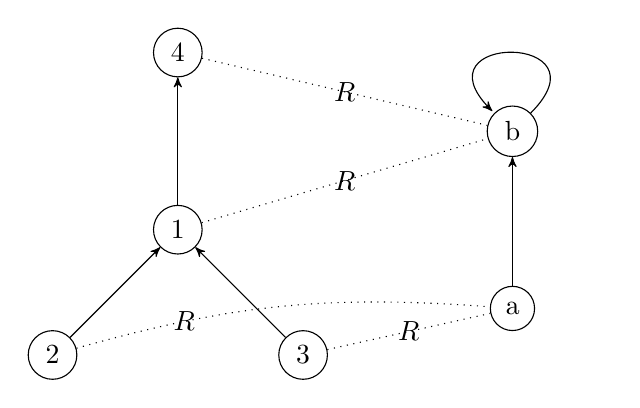
\begin{tikzpicture}[>=stealth',node distance=2.25cm]
\node [draw,circle] (1) {1};
\node [draw,circle,below left of = 1] (2) {2};
\node [draw,circle,below right of = 1] (3) {3};
\node [draw,circle,above of = 1] (4) {4};

\node [draw,circle,right of = 1,xshift=2cm,yshift=-1cm] (a) {a};
\node [draw,circle,above of = a] (b) {b};

\path (1) edge[->] (4)
		   (2) edge[->] (1)
		   (3) edge[->] (1)
		   (a) edge[->] (b)
  		   (b) edge[->,loop] (b)
		   (1) edge [dotted] node {$R$} (b)
		   (4) edge [dotted] node {$R$} (b)
		   (2) edge [dotted,bend left=10] node[near start] {$R$} (a)
		   (3) edge [dotted] node {$R$} (a);
\end{tikzpicture}
	\caption{Graph homomorphism. There is a relation $R$ that maps nodes of the left graph to the nodes of the right graph which keeps the connection of the right graph.}
	\label{fig:homomorphism}
\end{figure}

\paragraph{Graph summary.}

We call a graph $\mathcal{S}$ for which a graph $G$ is \emph{homomorphic} to --- the \emph{summary} of $G$ \cite{campinas:2012:dexa}. Indeed, the summary being homomorph to $G$ retain by definition the paths in the graph described in the property~(\ref{sprop-path}). Both graph share the set of labels $\mathcal{L}$, thus meeting the property~(\ref{sprop-voc}) of a summary.

\begin{definition}[Graph Summary]
Let $G=\left\langle V, A, l_V \right\rangle$ and $\mathcal{S}=\left\langle \mathcal{W}, \mathcal{B}, l_\mathcal{W} \right\rangle$ be two graphs such that their set of nodes are distinct, i.e., $V \cap \mathcal{W} = \emptyset$. Both graphs share the same set of labels $\mathcal{L}$. Let $R \subseteq V \times \mathcal{W}$ be a binary relation, and we call $R$ the \emph{summarisation relation}.
If $G$ is homomorphic to $\mathcal{S}$ then the graph $\mathcal{S}$ is a summary of $G$.
\end{definition}

\begin{remark}
From this point on, we shall differentiate between the nodes and edges of $G$ from those of $\mathcal{S}$ by calling a node of the summary a \emph{sumnode}, and an edge a \emph{sumedge}. Unless stated explicitly, the terms node and edge refer to the components of the entity graph $G$.
\end{remark}

Figure~\ref{fig:basic-summary} depicts a possible summary for a graph. The dotted lines illustrate the summarisation relation $R$, where we have for example $(a, S_1) \in R$ and $(John, S_3) \in R$.

\begin{figure}
	\centering
	\resizebox{.7\textwidth}{!}{
		\begin{tikzpicture}[>=stealth',->,node distance=2.5cm]
%% graph
\node[draw,circle] (a) {a};
\node[draw,circle,above left of = a,xshift=.5cm] (aage) {42};
\node[draw,circle,above right of = a,xshift=-.5cm] (aname) {John};

\node[draw,circle,below of = a] (b) {b};
\node[draw,circle,above left of = b,xshift=.5cm] (bage) {33};
\node[draw,circle,above right of = b,xshift=-.5cm] (bname) {Alice};

\coordinate (gx) at ($ (aage) + (-.75,.75) $);
\coordinate (gy) at ($ (bname) + (.95,-2.4) $);
\draw[rounded corners,dashed]  (gx) node[yshift=.3cm,xshift=1cm] {Graph $G$} rectangle (gy);

\path[every node/.style={fill=white,font=\footnotesize}]
(b) edge node {knows} (a)
(a) edge node {age} (aage)
(a) edge node {name} (aname)
(b) edge node {age} (bage)
(b) edge node {name} (bname)
;

%% summary
\node[draw,circle,right of = a,xshift=4.5cm,yshift=-1cm] (s) {$S_1$};
\node[draw,circle,above left of = s,xshift=.5cm] (sage) {$S_2$};
\node[draw,circle,above right of = s,xshift=-.5cm] (sname) {$S_3$};

\coordinate (sx) at ($ (sage) + (-.75,.75) $);
\coordinate (sy) at ($ (sname) + (.95,-3.5) $);
\draw[rounded corners,dashed]  (sx) node[yshift=.3cm,xshift=1.4cm] {Summary $\mathcal{S}$} rectangle (sy);

\path[every node/.style={font=\footnotesize}]
(s) edge[loop below] node {knows} (s)
(s) edge node[fill=white] {age} (sage)
(s) edge node[fill=white] {name} (sname)
;

\path[every node/.style={fill=white,font=\footnotesize},dotted]
(aage) edge[near end,bend right=10] node {$R$} (sage)
(bage) edge[bend left=10] node[near end] {$R$} (sage)
(aname) edge[near start,bend left=7] node {$R$} (sname)
(bname) edge node[near start] {$R$} (sname)
(a) edge[bend left=5] node {$R$} (s)
(b) edge node {$R$} (s)
;

\end{tikzpicture}
	}
	\caption{A graph and a possible summary. Dotted lines labelled $R$ represent the summarisation relation that maps nodes in the graph $G$ to sumnodes in $\mathcal{S}$.}
	\label{fig:basic-summary}
\end{figure}
%\begin{remark}
%Since the summarisation relation $R$ is a binary relation, we use the shorthand $R(u)$ to say that there exists a node $x \in \mathcal{W}$ such that $(u, x) \in R$, with $x = R(u)$.
%\end{remark}

%\begin{definition}[Graph Summary]
%Let $G=\left\langle V, A, l_V \right\rangle$ be a graph, and $R \subseteq V \times \mathcal{W}$ be a summarisation relation. The graph summary $\mathcal{S}=\left\langle \mathcal{W}, \mathcal{B}, l_\mathcal{W} \right\rangle$ of $G$ is defined as:
%\begin{enumerate}
%\item $\mathcal{W} = \left\lbrace y \mid (u,y) \in R \right\rbrace$;
%\item $\mathcal{B} \subseteq \left\lbrace \left(x, \alpha, y\right) \mid \exists (u,x) \in R \wedge \exists (v,y) \in R, \alpha \in \mathcal{L}^A \right\rbrace$.
%\end{enumerate}
%$l_\mathcal{W} : \mathcal{W} \mapsto \mathcal{L}_\mathcal{W}$ is a sumnode labelling function.
%\end{definition}

%\paragraph{Definition of a summary.}
%
%We use the symbol $\leftrightsquigarrow$ to express that a node of an entity graph $G$ is mapped to a sumnode of a summary $\mathcal{S}$ based on some features of the node.
%The Figure~\ref{fig:classes-summary} depicts a summary of the graph in the Figure~\ref{fig:graph} where the relation $R_t$ considers the set of types co-occurring in the graph. The table indicates the mappings by $R_t$ of the nodes in $V$, e.g., the nodes $N_1$ and $N_2$ are mapped to the sumnode $S_1$ since both connect to $Person$ via the type attribute. The summarisation relation $R_t$ is defined as:
%$$
%R_t = \left\lbrace (u, x) \in V \times \mathcal{W} \mid x \leftrightsquigarrow types(u) \right\rbrace
%$$
%\todo{review the definition of this notation. This may warrant a new definition.}

%The $\sim_t$-equivalence class ${[N_1]}^{\sim_t}$ contains the nodes $\left\lbrace N_1, N_2 \right\rbrace$ of $G$, since both connect to $Person$ via the type attribute.
%The concepts \emph{path}, \emph{type}, and \emph{attribute} introduced in the Section~\ref{sec:data-graph} hold for a summary.
%For example, we have for the node $[N_1]^{\sim_a}$ in the Figure~\ref{fig:attributes-summary} $types([N_1]^{\sim_a}) = \left\lbrace Person \right\rbrace$ and $attributes([N_1]^{\sim_a}) = \left\lbrace works, lives, name \right\rbrace$.
%\begin{definition}[Summary]
%Let $\sim$ be an equivalence relation and $G^\sim = \left\langle V^\sim, A^\sim, l_V^\sim \right\rangle$ be the $\sim$-summary of $G$, where $l_V^\sim$ be a $\sim$-equivalence class labelling function. The nodes $V^\sim$ are the $\sim$-equivalence classes on nodes of $G$ such that $V^\sim=\left\lbrace [x]^\sim : x \in V \right\rbrace$, with $[x]^\sim=\left\lbrace y \in V : y \sim x \right\rbrace$ the $\sim$-equivalence class of $x$. For every edge $x \overset{\alpha}{\rightarrow} y$ of $G$, there is an edge $[x]^\sim \overset{\alpha}{\rightarrow} [y]^\sim$ in $G^\sim$.
%\end{definition}

\paragraph{Partial relation.}

Depending on the definition of the summarisation relation $R$ some nodes of the graph do not have any mapping because they miss required features. For example, the node $N_0$ in Figure~\ref{fig:graph} does not have a $type$ edge; it has then no mapping for the previous relation $R_t$ that considers the set of types of a node as depicted in the Figure~\ref{fig:classes-summary}. As such, the relation $R$ is a \emph{partial relation}, where only a subset $V' \subseteq V$ has mappings; for the rest, it is \emph{undefined}. In the graph summary, we represent the set of undefined mappings with a sumnode labelled $\mathfrak{U}$.

\paragraph{Content abstraction.}

The purpose of a summary is to highlight the \emph{structure} of the graph, which is defined by the properties and types. Content information does not pertain the structure of the data, but only individual entities. Therefore, we abstract the summary from the content by mapping content nodes to a ``sink'' sumnode that we label as $\varnothing$. For example, the node labelled $Ireland$ in the Figure~\ref{fig:graph} is mapped to $\varnothing$. In RDF graphs, literals are mapped to the sink sumnode.


\begin{figure}
	\centering
	\begin{minipage}{.7\textwidth}
		\resizebox{\textwidth}{!}{
			\usetikzlibrary{arrows}

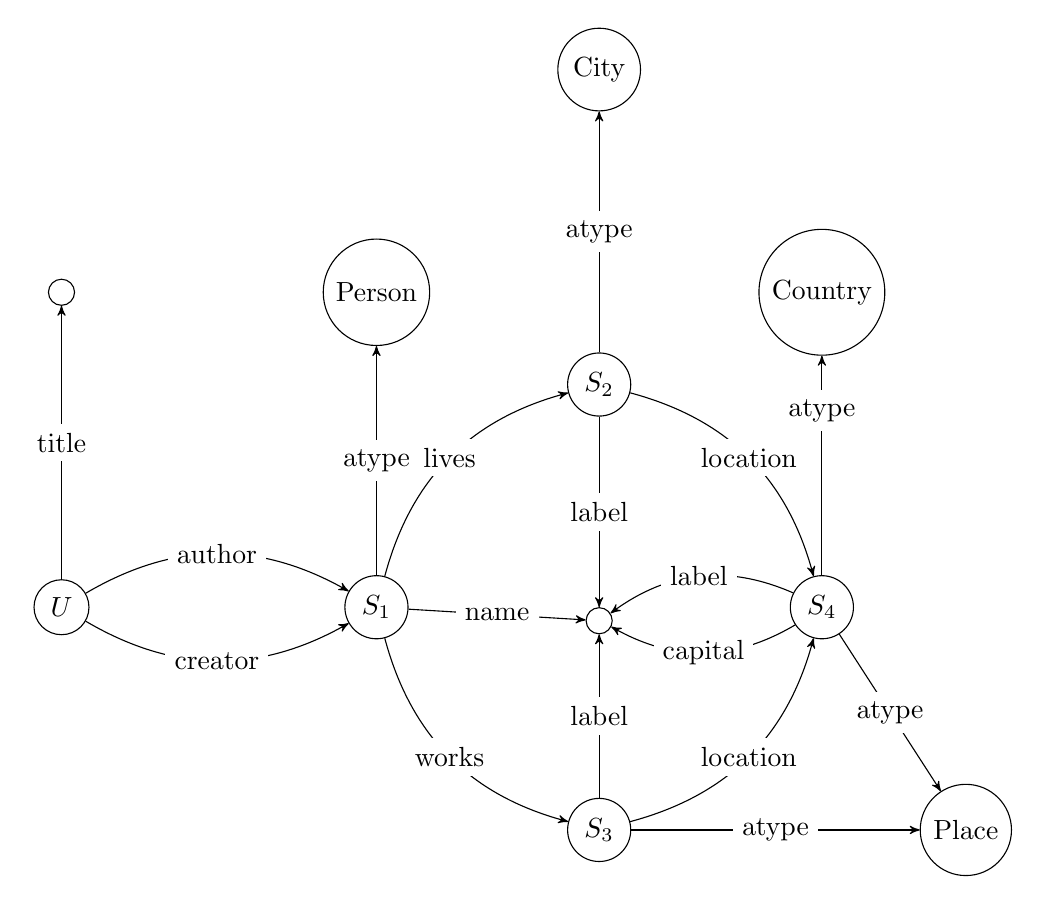
\begin{tikzpicture}[->,>=stealth',node distance=4cm]
\node [draw,circle] (b) {$\mathfrak{U}$};
\node [draw,circle,right of = b] (h1) {$S_1$};
\node [draw,circle,above right of = h1] (h2) {$S_2$};
\node [draw,circle,below right of = h1] (h3) {$S_3$};
\node [draw,circle,above right of = h3] (h4) {$S_4$};
\node [draw,circle,above of = h1] (person) {Person};
\node [draw,circle,above of = h2] (city) {City};
\node [draw,circle,above of = h4] (country) {Country};
\node [draw,circle,below right of = h4,xshift=-1cm] (place) {Place};
\node [draw,circle,above of = b] (c1) {$\varnothing$};
\node [draw,circle,below of = h2,yshift=1cm] (c2) {$\varnothing$};

\path
(b) edge node[fill=white] {title} (c1)
(h1) edge node[fill=white] {name} (c2)
(h3) edge node[fill=white] {label} (c2)
(h2) edge node[fill=white] {label} (c2)
(h4) edge[bend right] node[fill=white] {label} (c2)
(h4) edge[bend left] node[fill=white] {capital} (c2)

(h1) edge node[fill=white] {\glssymbol{atype}} (person)
(h2) edge node[fill=white] {\glssymbol{atype}} (city)
(h4) edge node[near end,fill=white] {\glssymbol{atype}} (country)
(h4) edge node[fill=white] {\glssymbol{atype}} (place)
(h3) edge node[fill=white] {\glssymbol{atype}} (place)
(h1) edge[bend left] node[fill=white] {lives} (h2)
(h1) edge[bend right] node[fill=white] {works} (h3)
(h2) edge[bend left] node[fill=white] {location} (h4)
(h3) edge[bend right] node[fill=white] {location} (h4)
(b) edge[bend right] node[fill=white] {creator} (h1)
(b) edge[bend left] node[fill=white] {author} (h1)
;
\end{tikzpicture}
		}
	\end{minipage}
	\quad
	\begin{minipage}[h]{.25\textwidth}
		\centering
		\caption*{$R_t\left(V, \mathcal{W}\right)$}
		\begin{tabular}{lc@{\hs}l}
			\toprule
			$V$ & \phantom{a} & $\mathcal{W}$ \\
			\cmidrule{1-1} \cmidrule{3-3}
			$N_0$ & \phantom{a} & $\mathfrak{U}$ \\
			$N_1$, $N_2$ & \phantom{a} & $S_1$ \\
			$N_3$ & \phantom{a} & $S_2$ \\
			$N_4$, $N_5$ & \phantom{a} & $S_3$ \\
			$N_6$, $N_7$ & \phantom{a} & $S_4$ \\
			\bottomrule
		\end{tabular}
	\end{minipage}
	\caption{Summary of the graph in Figure~\ref{fig:graph} with the summarisation relation $R_t$. The table indicates the mappings by $R_t$. The content in $G$ is abstracted by the sumnode $\varnothing$.}
	\label{fig:classes-summary}
\end{figure}

%We define the \emph{sink equivalence class} as the set of sink nodes, e.g., the node labelled $Ireland$ in the Figure~\ref{fig:graph} is part of this set. We remark that in the RDF data model, \emph{literals} are part of the sink equivalence class.
%\begin{definition}[Sink Equivalence Class]
%The set of sink nodes in $G$ is represented by the sink equivalence class $[\emptyset]=\left\lbrace x \in V : \not \exists (x, \alpha, y) \in A \right\rbrace$ in $G^\sim$.
%\end{definition}
%
%Depending on the $\sim$-equivalence, there can be nodes that do not have the required features to be assigned to a $\sim$-equivalence class. We define $B^\sim$ the \emph{blank $\sim$-equivalence class} as the set of such nodes of $G$, e.g., the node $N_0$ in the Figure~\ref{fig:graph} is assigned to the node $B^{\sim_t}$ in the Figure~\ref{fig:classes-summary}.
%\begin{definition}[Blank $\sim$-Equivalence Class]
%The set of nodes in $G$ for which there is no $\sim$-equivalent class is equal to the blank $\sim$-equivalence class $B^\sim$, i.e., $B^\sim=\left\lbrace x \in V : \forall y \in V, x \not \sim y \right\rbrace$.
%\end{definition}

\subsection{Precise Graph Summary}

The purpose of a summary is to mirror the structure of the graph while being significantly smaller. Therefore, the summary can substitute the graph and improve the performance of applications. How well the summary mirrors the graph is then of high importance. From a structural perspective, a summary is precise if it is undiscernable from the original graph.

Although the structure of the graph is preserved in the summary by definition of graph homomorphism, the structure of the summary may not exactly reflect the structure of the graph. Indeed, a summary may have paths that are not present in the original graph $G$, as depicted in the Figure~\ref{fig:homomorphism}.

Indeed, we remark that although the structure of the graph $G$ is kept in the summary, the inverse may not hold true. The Figure~\ref{fig:homomorphism} depicts a loop on the $b$ node; although there is an edge from $1$ to $4$, there is no edge in the opposite direction.\\
%In Section~\ref{chap03:sec:quality} we study the precision of an \emph{approximate} graph summary.

A summary is built from a graph based on a summarisation relation that maps each node of that graph to a sumnode, i.e., a node of the summary. An edge $(u, \alpha, v) \in A$ is mapped to a sumedge by definition of the graph homomorphism. Several paths in the graph may be mapped to a same path on the summary. We introduce the \emph{summary path instance} as the set of nodes in the graph which mappings form a path in the summary. For example, if we consider the summary in Figure~\ref{fig:classes-summary} built with the summarisation relation $R_t$, the set $\{N_1, N_3, N_6\}$ in an instance of the path $(S_1, lives, S_2) \in \mathcal{W} \wedge (S_2, lives, S_4) \in \mathcal{W}$ in that summary; indeed, we have $(N_1, S_1) \in R_t$, $(N_3, S_2) \in R_t$, and $(N_6, S_4) \in R_t$.

\begin{definition}[Summary Path Instance]
Let $G=\left\langle V, A, l_V \right\rangle$ be a graph, and $\mathcal{S} = \left\langle \mathcal{W}, \mathcal{B}, l_{\mathcal{W}} \right\rangle$ be the summary of $G$ according to the summarisation relation $R \subseteq V \times \mathcal{W}$.

Let $p = (x_1, \alpha_1, x_2) \in \mathcal{B} \wedge \cdots \wedge (x_n, \alpha_n, x_{n+1}) \in \mathcal{B}$ be a path in the summary $\mathcal{S}$ with $(x_1, \cdots, x_{n+1}) \in \mathcal{W}^{n+1}$.
We call the set $\{ u_1, \cdots, u_{n+1} \}$ an instance of the summary path $p$ if each node $u_i \in V$ is mapped to a sumnode $x_i$ of $p$, i.e.,:
$$
\forall i \in \left[1, n\right] \; (u_i, x_i) \in R
$$
\end{definition}

In the previous example, we remark that the summary path instance $\{N_1, N_3, N_6\}$ given for $(S_1, lives, S_2) \in \mathcal{W} \wedge (S_2, lives, S_4) \in \mathcal{W}$ in Figure~\ref{fig:classes-summary} is not the only one. Indeed, there are three more instances possible, i.e., $\{N_1, N_3, N_7\}$, $\{N_2, N_3, N_6\}$, and $\{N_2, N_3, N_7\}$. However, two out of those four do not form a path in the graph in Figure~\ref{fig:graph}, i.e., the sets $\{N_1, N_3, N_7\}$ and $\{N_2, N_3, N_7\}$. We call a summary \emph{precise} if there is no such case.

\begin{definition}[Precise Graph Summary]
Let $G=\left\langle V, A, l_V \right\rangle$ be a graph, and $\mathcal{S} = \left\langle \mathcal{W}, \mathcal{B}, l_{\mathcal{W}} \right\rangle$ be the summary of $G$ according to the summarisation relation $R \subseteq V \times \mathcal{W}$.
We say that the summary $\mathcal{S}$ is \emph{precise} if each summary path instance forms a path that does exist in the graph $G$.
\end{definition}

\subsubsection{Bisimulation}
\label{chap:summary:bisim}

The bisimulation~\cite{park:1981:cai} is a notion of concurrency that studies the equality of processes.
%It can be seen as a weaker formulation of graph isomorphism in that it defines many-to-one mappings.
A bisimulation is a binary relation on $V$ that relates two nodes of the graph if itself and its inverse are \emph{simulations}.

If we consider two nodes $(u, v) \in V$, a simulation $R$ is a relation that states that for every edge $(u, \alpha, x) \in A$, there exists an edge $(v,\alpha, y) \in A$ such that there is also a simulation between the nodes $x$ and $y$. Intuitively, $(u,v) \in R$ communicates that the node $v$ can \emph{substitute} the node $u$ since all the outgoing paths from $u$ match those from $v$. A bisimulation is stronger as it states that the relation must be \emph{symmetric} as well, thus ensuring that either node may substitute the other.

Figure~\ref{fig:bisimulation} depicts the simulation relation $R$ between nodes $E_0$ and $E'_0$ such that $(E_0, E'_0) \in R$; this illustrates that:
\begin{enumerate}
	\item for every outgoing edge from $E_0$, there is also such an edge from $E'_0$; and
	\item there is a simulation between the nodes thus reached $E_i$ and $E'_i$, i.e., $(E_i, E'_i) \in R$.
\end{enumerate}
If for the node $E'_0$ the previous two points hold as well, then the binary relation $R$ is actually a \emph{bisimulation}.
%Two nodes are said \emph{bisimilar} if there is a bisimulation relation between the two.
%Sink nodes are always bisimilar.

\begin{definition}[Bisimulation]
Let $G=\left\langle V, A, l_V \right\rangle$ be a graph and $\sim \subseteq V \times V$ a binary relation on $V$.
The relation $\sim$ is a bisimulation if $\forall (x,y) \in\; \sim$:
\begin{equation*}
\forall (x, \alpha, x') \in A\; \exists (y, \alpha, y') \in A \wedge (x',y') \in\; \sim
\label{eq:b1}
\end{equation*}
The converse must hold as well, i.e.:
\begin{equation*}
\forall (y, \alpha, y') \in A\; \exists (x, \alpha, x') \in A \wedge (x',y') \in\; \sim
\label{eq:b2}
\end{equation*}
\end{definition}

\begin{remark}
Two nodes $(u, v) \in V^2$ are said \emph{bisimilar} if $(u, v) \in \sim$.
\end{remark}

\begin{figure}
	\centering
	\resizebox{.5\textwidth}{!}{
		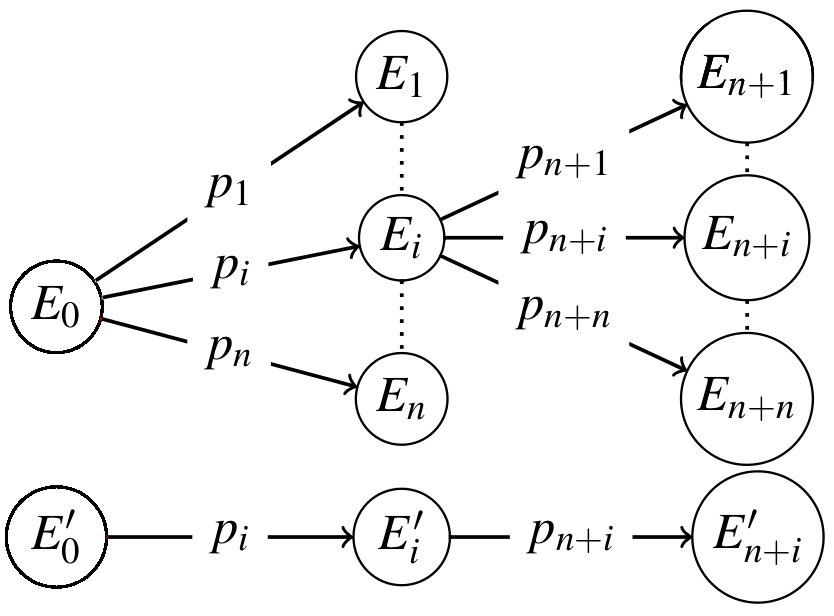
\includegraphics{04-summary/figures/bisimulation}
	}
	\caption{Simulation relation}
	\label{fig:bisimulation}	
\end{figure}

The coinductive aspect of the definition ensures that two nodes are bisimilar if their \emph{outgoing} paths are the same. Kaushik et al.~\cite{kaushik:2002:cib} propose the \emph{forward-and-backward} (f\&b)-bisimulation which extends the definition by considering incoming edges in addition to the outgoing ones. Since a summary deals with the graph's structure given by the relationships of attributes and types, we introduce the type as an additional requirement.

In addition to the requirements of a f\&b-bisimulation between two nodes, we consider their type information. We define the \emph{fbt-bisimulation} as the f\&b-bisimulation that ensures that nodes are equivalent with regards to their type as well.

\begin{definition}[FBT-Bisimulation]
Let $G=\left\langle V, A, l_V \right\rangle$ be a graph and $(\sim_f, \sim_b, \sim_t) \subseteq (V \times V)^3$ be three equivalence relations on $V$.
The relation $\approx_t \subseteq V \times V$ on $V$ is a fbt-bisimulation if $\forall (x,y) \in\; \approx_t$, we have $(x,y) \in\; \sim_f$, $(x,y) \in\; \sim_b$ and $(x,y) \in\; \sim_t$ such that:
\begin{enumerate}
\item $\sim_f$ is a forward bisimulation such that:
$$
\begin{aligned}
\forall (x, \alpha, x') \in A&\; \exists (y, \alpha, y') \in A \wedge (x',y') \in\; \sim_f \\
\text{conversely,}\;\; \forall (y, \alpha, y') \in A&\; \exists (x, \alpha, x') \in A \wedge (x',y') \in\; \sim_f
\end{aligned}
$$

\item $\sim_b$ is a backward bisimulation such that:
$$
\begin{aligned}
\forall (x^{-1}, \alpha, x) \in A&\; \exists (y^{-1}, \alpha, y) \in A \wedge (x^{-1}, y^{-1}) \in\; \sim_b \\
\text{conversely,}\;\; \forall (y^{-1}, \alpha, y) \in A&\; \exists (x^{-1}, \alpha, x) \in A \wedge (x^{-1}, y^{-1}) \in\; \sim_b
\end{aligned}
$$

\item $\sim_t$ preserves the types such that:
$$
\begin{aligned}
\forall (x, \gls{atype}, t) \in A&\; \exists (y, \gls{atype}, t) \in A \\
\text{conversely,}\;\; \forall (y, \gls{atype}, t) \in A&\; \exists (x, \gls{atype}, t) \in A
\end{aligned}
$$

\end{enumerate}
\end{definition}

\subsubsection{Bisimulation Summary Construction}

Since the bisimulation is an equivalence relation, we can create equivalence classes defined as $[x] = \left\lbrace x \in V \mid y \in V,\; x \sim y \right\rbrace$; a class is the set of nodes that are bisimilar. An equivalence class is then exactly a sumnode of the summary. The summarisation relation is in this case a one-to-one mapping of the equivalence class to the sumnode.

\begin{definition}[Bisimulation Summary]
Let $G=\left\langle V, A, l_V \right\rangle$ and $\mathcal{S}_{fbt} = \left\langle \mathcal{W}_{fbt}, \mathcal{B}_{fbt}, l_{\mathcal{W}_{fbt}} \right\rangle$ be two graphs. Let $\approx_t \subseteq V \times V$ be a fbt-bisimulation relation.

The set of nodes $\mathcal{W}_{fbt}$ contains as many elements as there are equivalence classes as per the fbt-bisimulation relation:
$$
\lvert \mathcal{W}_{fbt} \rvert = \lvert \left\lbrace [x] \mid \exists y \in V\; x \approx_t y \right\rbrace \rvert
$$

We call $\mathcal{S}_{fbt}$ the bisimulation summary of $G$ according to the summarisation relation $R_{fbt} \subseteq V \times \mathcal{W}_{fbt}$ defined as a one-to-one mapping between the set of equivalence classes and the set $\mathcal{W}_{fbt}$:
$$
\begin{aligned}
R_{fbt} = \{ \left( u, x \right) \in V \times \mathcal{W}_{fbt} \mid & \forall v \in [u]\; \left( v, x \right) \in V \times \mathcal{W}_{fbt} \\
& \wedge \exists w \not \in [u]\; \exists y \in \mathcal{W}_{fbt} (w, y) \in V \times \mathcal{W}_{fbt} \wedge x \neq y \}
\end{aligned}
$$
\end{definition}

\begin{remark}
We note as $R_f$ and $R_b$ the summarisation relations which equivalence classes are based on the forward $\sim_f$ and backward $\sim_b$ bisimulations, respectively.
\end{remark}

The summary depicted on the Figure~\ref{fig:fbb-summary} with the bisimulation $R_{fbt}$ assigns an equivalence class to \emph{each} node of the graph in Figure~\ref{fig:graph}. In the running example, the only difference of the summary with the data graph is the content abstraction, e.g., the node \emph{Ireland} is represented by the node $\varnothing$.

In order to compute this summary, the algorithm proposed in \cite{Paige:1987:TPR:37185.37186} is generally used. It offers a $O\left( \vert A \vert \times log\left( \vert V \vert \right) \right)$ complexity for the computation of the bisimulation. We note that the algorithm starts from an existing partitioning of the graph. Then, the partitions are refined iteratively until all nodes in a partition are bisimilar.% The computation of the $\sim_{fbt}$-summary is achieved by applying over the $\sim_{fb}$ graph a slightly modified version of the \cite{Paige:1987:TPR:37185.37186} algorithm, in order to account for the incoming edges in the $\sim_{bb}$ definition. We remark that the complexity of all other algorithms are lower than the complexity of $\sim_{b}$.
%In addition, the \cite{Paige:1987:TPR:37185.37186} algorithm requires more than one iteration over the data graph, the number of iterations equal to the data graph diameter in the worst case. Iterative algorithms are sub-optimal for shared-nothing infrastructures, e.g., MapReduce. The reason is the data graph needs to be read and written at each iteration, leading to an important IO load. Therefore, one pass algorithms can better scale to large and heterogeneous data graphs using shared-nothing infrastructures.

\begin{figure}
	\centering
	\begin{minipage}{.75\textwidth}
		\resizebox{\textwidth}{!}{
			\usetikzlibrary{arrows}

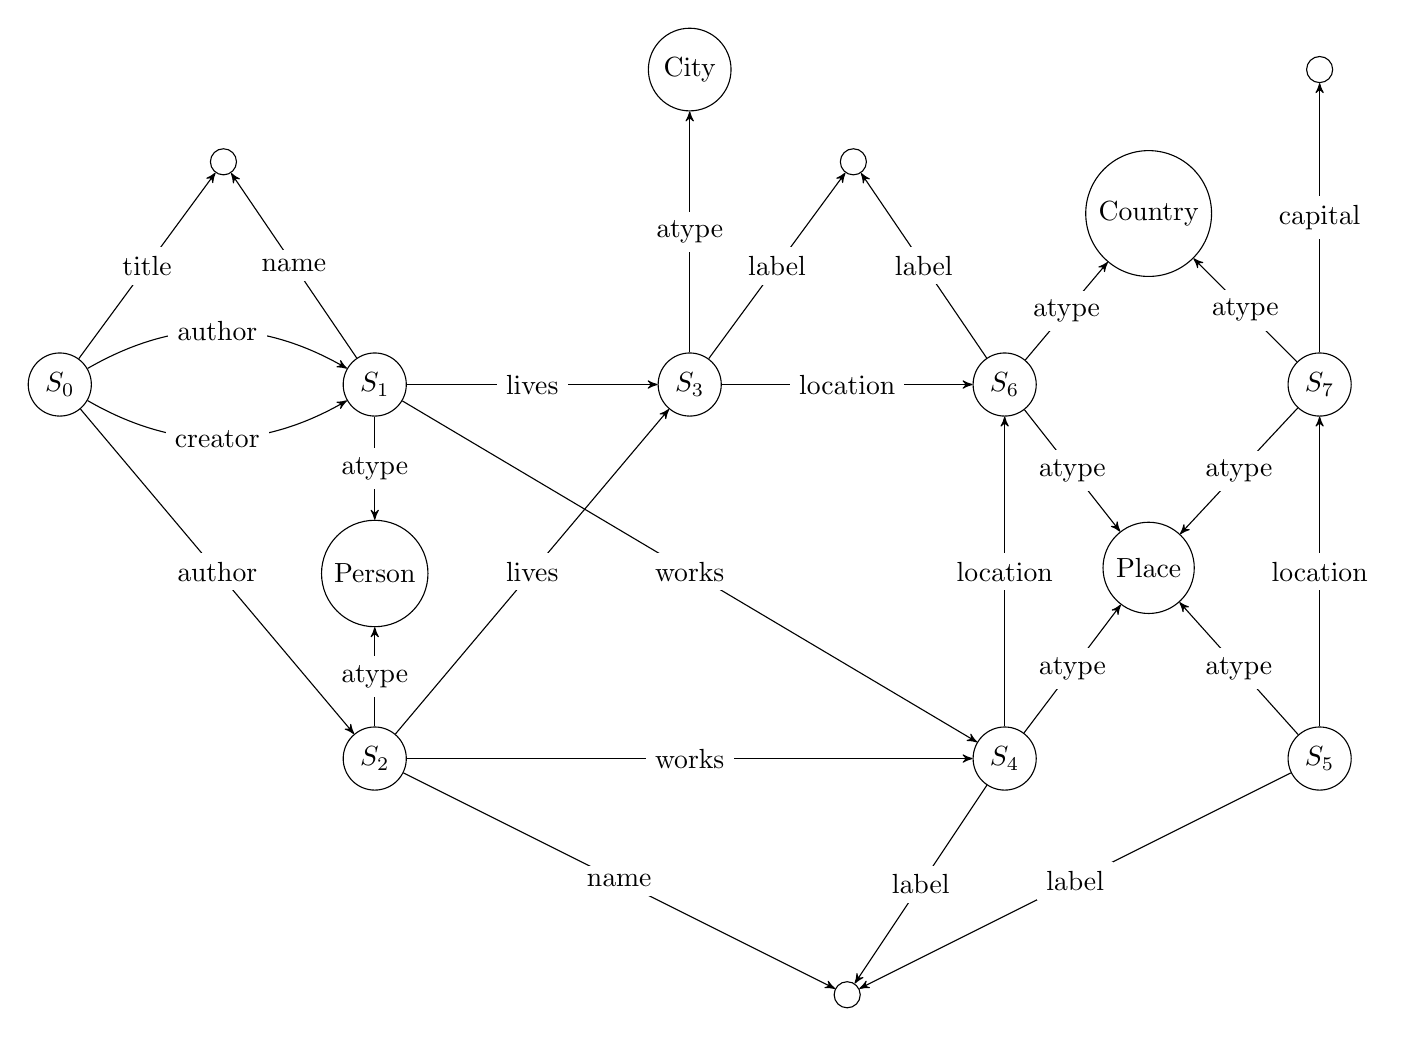
\begin{tikzpicture}[->,>=stealth',node distance=4cm]

\node [draw,circle] (n0) {$S_0$};
\node [draw,circle,right of = n0] (n1) {$S_1$};
\node [draw,circle,below of = n1,yshift=-.75cm] (n2) {$S_2$};
\node [draw,circle,right of = n1] (n3) {$S_3$};
\node [draw,circle,right of = n3] (n6) {$S_6$};
\node [draw,circle,below of = n6,yshift=-.75cm] (n4) {$S_4$};
\node [draw,circle,right of = n6] (n7) {$S_7$};
\node [draw,circle,right of = n4] (n5) {$S_5$};

\node [draw,circle,above of = n3] (city) {City};
\node [draw,circle,below right of = n6,xshift=-1cm,yshift=.5cm] (place) {Place};
\node [draw,circle,above of = place,yshift=.5cm] (country) {Country};
\node [draw,circle,above of = n2,yshift=-1.65cm] (person) {Person};

\node [draw,circle,above right of = n0,xshift=-.75cm] (s1) {$\varnothing$};
\node [draw,circle,above right of = n3,xshift=-.75cm] (s2) {$\varnothing$};
\node [draw,circle,below of = n4,yshift=1cm,xshift=-2cm] (s3) {$\varnothing$};
\node [draw,circle,above of = n7] (s4) {$\varnothing$};

\path
(n0) edge[bend right] node[fill=white] {creator} (n1)
(n0) edge[bend left] node[fill=white] {author} (n1)
(n0) edge node[fill=white] {author} (n2)
(n1) edge node[fill=white] {lives} (n3)
(n1) edge node[fill=white] {works} (n4)
(n2) edge node[fill=white] {lives} (n3)
(n2) edge node[fill=white] {works} (n4)
(n3) edge node[fill=white] {location} (n6)
(n4) edge node[fill=white] {location} (n6)
(n5) edge node[fill=white] {location} (n7)
(n4) edge node[fill=white] {\glssymbol{atype}} (place)
(n5) edge node[fill=white] {\glssymbol{atype}} (place)
(n6) edge node[fill=white] {\glssymbol{atype}} (place)
(n7) edge node[fill=white] {\glssymbol{atype}} (place)
(n6) edge node[fill=white] {\glssymbol{atype}} (country)
(n7) edge node[fill=white] {\glssymbol{atype}} (country)
(n1) edge node[fill=white] {\glssymbol{atype}} (person)
(n2) edge node[fill=white] {\glssymbol{atype}} (person)
(n3) edge node[fill=white] {\glssymbol{atype}} (city)
(n0) edge node[fill=white] {title} (s1)
(n1) edge node[fill=white] {name} (s1)
(n3) edge node[fill=white] {label} (s2)
(n6) edge node[fill=white] {label} (s2)
(n2) edge node[fill=white] {name} (s3)
(n4) edge node[fill=white] {label} (s3)
(n5) edge node[fill=white] {label} (s3)
(n7) edge node[fill=white] {capital} (s4)
;
\end{tikzpicture}
		}
	\end{minipage}
	\quad
	\begin{minipage}[h]{.2\textwidth}
		\centering
		\caption*{$R_{fbt}\left(V, \mathcal{W}\right)$}
		\begin{tabular}{lc@{\hs}l}
			\toprule
			$V$ & \phantom{a} & $\mathcal{W}$ \\
			\cmidrule{1-1} \cmidrule{3-3}
			$N_0$ & \phantom{a} & $S_0$ \\
			$N_1$ & \phantom{a} & $S_1$ \\
			$N_2$ & \phantom{a} & $S_2$ \\
			$N_3$ & \phantom{a} & $S_3$ \\
			$N_4$ & \phantom{a} & $S_4$ \\
			$N_5$ & \phantom{a} & $S_5$ \\
			$N_6$ & \phantom{a} & $S_6$ \\
			$N_7$ & \phantom{a} & $S_7$ \\
			\bottomrule
		\end{tabular}
	\end{minipage}
	\caption{Summary of the graph in Figure~\ref{fig:graph} with bisimulation $R_{fbt}$ as the summarisation relation. The table indicates the mappings by $R_{fbt}$. The content in $G$ is abstracted by the sumnode $\varnothing$.}
	\label{fig:fbb-summary}
\end{figure}

\subsection{Approximate Graph Summary}
\label{sec:approximate}

%A graph summary is built so that it describes the structure of the graph, providing similar benefits as a relational schema does for a database, which we discuss in Section~\ref{chap03:sec:gschema}.
In general, we find in Web Data a heterogeneous use of vocabularies, where several different ontologies can be used within the same dataset, in ways that might not have been intended for. Web Data presents a complex graph structure that varies greatly from dataset to dataset.

In addition, Web Data is composed of user-created content which quality is not assessed, e.g., use of an appropriate ontology, typographic errors when editing, incorrect description of an entity, etc. This quality issue, combined with the heterogeneity of the graph, is an obstacle towards the generation of a precise summary. Indeed, attempting to record every single path would require a summary so large that its benefits would be nullified. Therefore, we present in this section \emph{approximate} graph summaries.

\subsubsection{Heterogeneous Graph Structure}

We investigate the direction of \emph{approximate} summarisation for the creation of a graph summary. DataGuides~\cite{goldman1997dataguides} were proposed to index the structure of data following the OEM model.
%A requirement of the approach is that every path in the DataGuide appears in the original graph as well.
The creation of a DataGuide is equivalent to the conversion of a non-deterministic finite automaton to a deterministic finite automaton.
Due to heterogeneous structure of the data, the size of a DataGuide grows exponentially, becoming larger than the original data as noted by Goldman et al.~\cite{goldman1999approximate}.

We created in~\cite{campinas:2011:eos} a dataset based on Sindice\footnote{\url{http://sindice.com}}'s collection for the task of entity-oriented search. The Figure~\ref{fig:onto-dist} depicts the distribution of the frequency of ontologies used across documents, i.e., the probability for an ontology to be used in exactly $n$ documents. The distribution shows a power-law distribution following a Zipf function with a slope of $\alpha = 2.27$.
%For example, one ontology (\url{http://purl.org/dc/terms/}) is used in more than 150 million documents and another one (\url{http://www.w3.org/2006/vcard/ns\#}) is used in more than 64 millions documents.

This investigation has showed that most ontologies (99\%) are used only once. However, the distribution tail is sparse, suggesting that a few ontologies are used in a large proportion of documents.
This result strengthens our belief that it is not a viable option in many cases for a graph summary to retain every path and combinations of paths that occur in an entity graph.

\begin{figure}
	\centering
	\begin{tikzpicture}
    \begin{loglogaxis}[
                grid=major,
                        xlabel=number of documents (\emph{log}),
                        ylabel=probability (\emph{log}),
                ]       
        \addplot[red, domain=1:100,ultra thick] {0.00257344864/(x^1.913581)};
        \addlegendentry{$\alpha =  1.91$}       
        \addplot+[only marks, mark size=1pt,mark=star, blue] table[x index=1,y index=0] {04-summary/experiments/basic-namespace-stats-probability};
	\end{loglogaxis}
\end{tikzpicture}
	\caption{Ontology probability distribution}
	\label{fig:onto-dist}
\end{figure}

%\begin{itemize}
%\item Scalability issues (computation performance + summary size) of current graph summarisation
%\item Approximate definition of graph summarisation.
%\end{itemize}

\subsubsection{Approximate Summarisation Relation}

A graph summary can be constructed based on various features of the data. We present here some summarisation relations that consider the following features of the graph:
\begin{itemize}
	\item the predicate URI;
	\item the type URI; and
	\item the direction of links, i.e., incoming or outgoing.
\end{itemize}
We report in Table~\ref{tab:sumrel} the relations along with the name of the summary that it generates.

\begin{labeling}{$R_{ioat}$ \textbf{relation.}}
\item[$R_{st}$ \textbf{relation.}]

We define $R_{st}$ as the summarisation relation that maps a node according to its type. Formally:
$$
\begin{aligned}
R_{st} = \{ (u, x) \in V \times \mathcal{W}_{st} \mid &\; \exists (v,y) \in V \times \mathcal{W}_{st} \\
 & (u,\gls{atype},v) \in A \wedge (x,\gls{atype},y) \wedge l_V(v) = l_\mathcal{W}(y) \}
\end{aligned}
$$
The nodes $N_4$, $N_5$, $N_6$, and $N_7$ in the Figure~\ref{fig:graph} are mapped to a same sumnode since they all have \emph{Place} as a type. The $R_{st}$ relation may map a node to multiple sumnodes since an entity may have several types. For instance, the nodes $N_6$ and $N_7$ are also mapped to another sumnode since they both share the type \emph{Country}.

\item[$R_t$ \textbf{relation.}]

We define $R_t$ the relation that maps a node based on its set of types. Formally:
$$
R_t = \left\lbrace (u, x) \in V \times \mathcal{W}_t \mid types(u) = types(x) \right\rbrace
$$
The Figure~\ref{fig:classes-summary} depicts the $R_t$ summary of the graph in in the Figure~\ref{fig:graph}. The nodes $N_6$ and $N_7$ are mapped to the sumnode $S_4$ because they are both associated with the types \emph{Place} and \emph{Country}. The table indicates the mappings by $R_t$ of the nodes in $V$, e.g., the nodes $N_1$ and $N_2$ are mapped to the sumnode $S_1$ since both connect to $Person$ via the type attribute. It differs from $R_{st}$ since it considers the types of a node as \emph{set} rather than individually. Indeed, the node $N_6$ is mapped to two sumnodes under the relation $R_{st}$.

\item[$R_a$ \textbf{relation.}]

We define $R_a$ the relation that maps a node based on its set of predicates. Formally:
$$
R_a = \left\lbrace (u, x) \in V \times \mathcal{W}_a \mid attributes(u) = attributes(x) \right\rbrace
$$
The nodes $N_3$, $N_4$, and $N_5$ are $\sim_a$-equivalent because they share the same set of attributes, i.e., $\left\lbrace label, location, type \right\rbrace$. The graph in Figure~\ref{fig:attributes-summary} is the $\sim_a$-summary of the data graph in Figure~\ref{fig:graph}.

\begin{figure}
	\centering
	\begin{minipage}{.75\textwidth}
		\resizebox{\textwidth}{!}{
			\usetikzlibrary{arrows}

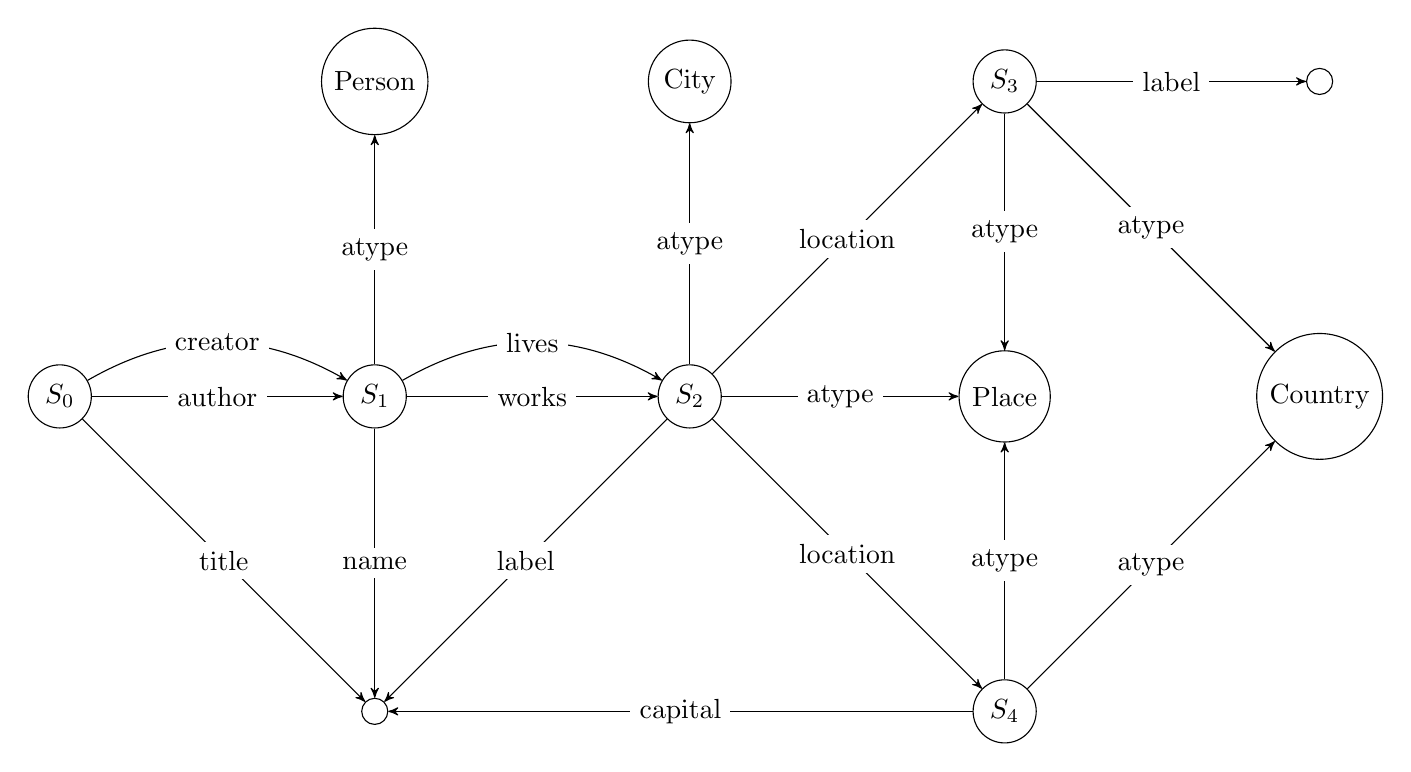
\begin{tikzpicture}[->,>=stealth',node distance=4cm]
\node [draw,circle] (n0) {$S_0$};
% \node (n0) [draw,thick,rectangle,inner sep=0] {
% \begin{tabular}{l}
% \multicolumn{1}{c}{$S_0$} \\
% \hline
% \\
% \hline
% - title
% \end{tabular}
% };

\node [draw,circle,right of = n0] (n1) {$S_1$};
% \node (n1) [draw,thick,rectangle,inner sep=0,right of = n0] {
% \begin{tabular}{l}
% \multicolumn{1}{c}{$S_1$} \\
% \hline
% - Person \\
% \hline
% - name
% \end{tabular}
% };

\node [draw,circle,above of = n1] (person) {Person};
\node [draw,circle,right of = n1] (n2) {$S_2$};
% \node (n2) [draw,thick,rectangle,inner sep=0,right of = n1] {
% \begin{tabular}{l}
% \multicolumn{1}{c}{$S_2$} \\
% \hline
% - City \\
% \hline
% - label
% \end{tabular}
% };

\node [draw,circle,right of = n2] (place) {Place};
\node [draw,circle,above of = place] (n3) {$S_3$};
% \node (n3) [draw,thick,rectangle,inner sep=0,above right of = n2] {
% \begin{tabular}{l}
% \multicolumn{1}{c}{$S_3$} \\
% \hline
% - Place \\
% - Country \\
% \hline
% - label
% \end{tabular}
% };

\node [draw,circle,above of = n2] (city) {City};
\node [draw,circle,below of = place] (n4) {$S_4$};
% \node (n4) [draw,thick,rectangle,inner sep=0,below right of = n2] {
% \begin{tabular}{l}
% \multicolumn{1}{c}{$S_4$} \\
% \hline
% - Place \\
% - Country \\
% \hline
% - capital
% \end{tabular}
% };

\node [draw,circle,right of = place] (country) {Country};
\node [draw,circle,below of = n1] (s1) {$\varnothing$};
\node [draw,circle,right of = n3] (s2) {$\varnothing$};

\path
(n0) edge node[fill=white] {author} (n1)
(n0) edge[bend left] node[fill=white] {creator} (n1)
(n1) edge node[fill=white] {\gls{atype}} (person)
(n1) edge node[fill=white] {works} (n2)
(n1) edge[bend left] node[fill=white] {lives} (n2)
(n2) edge node[fill=white] {\gls{atype}} (city)
(n2) edge node[fill=white] {location} (n3)
(n2) edge node[fill=white] {location} (n4)
(n2) edge node[fill=white] {\gls{atype}} (place)
(n3) edge node[fill=white] {\gls{atype}} (country)
(n4) edge node[fill=white] {\gls{atype}} (country)
(n3) edge node[fill=white] {\gls{atype}} (place)
(n4) edge node[fill=white] {\gls{atype}} (place)
(n0) edge node[fill=white] {title} (s1)
(n1) edge node[fill=white] {name} (s1)
(n2) edge node[fill=white] {label} (s1)
(n4) edge node[fill=white] {capital} (s1)
(n3) edge node[fill=white] {label} (s2)
;
\end{tikzpicture}
		}
	\end{minipage}
	\quad
	\begin{minipage}[h]{.2\textwidth}
		\centering
		\caption*{$R_a\left(V, \mathcal{W}\right)$}
		\resizebox{\textwidth}{!}{
		\begin{tabular}{lc@{\hs}l}
			\toprule
			$V$ & \phantom{a} & $\mathcal{W}$ \\
			\cmidrule{1-1} \cmidrule{3-3}
			$N_0$ & \phantom{a} & $S_0$ \\
			$N_1$, $N_2$ & \phantom{a} & $S_1$ \\
			$N_3$, $N_4$, $N_5$ & \phantom{a} & $S_2$ \\
			$N_6$ & \phantom{a} & $S_3$ \\
			$N_7$ & \phantom{a} & $S_4$ \\
			\bottomrule
		\end{tabular}}
	\end{minipage}
	\caption{Summary of the graph in Figure~\ref{fig:graph} with $R_a$. The table indicates the mappings by $R_a$. The content in $G$ is abstracted by the sumnode $\varnothing$.}
	\label{fig:attributes-summary}
\end{figure}

\item[$R_{at}$ \textbf{relation.}]

We define $R_{at}$ as the relation that maps a node based on its set of types and attributes. Formally:
$$
\begin{aligned}
R_{at} = \{ (u, x) \in V \times \mathcal{W}_{at} \mid &\; types(u) = types(x) \\
& \wedge attributes(u) = attributes(x) \}
\end{aligned}
$$
The nodes $N_1$ and $N_2$ are mapped to mapped to a same sumnode by $R_{at}$ because they are associated with the same type, i.e., \emph{Person}, and they have the same attributes, i.e., $\left\lbrace lives, name, type, works \right\rbrace$.

\item[$R_{ioa}$ \textbf{relation.}]

We define $R_{ioa}$ the relation based on the set of incoming and outgoing attributes; that is:
$$
\begin{aligned}
R_{ioa} =
\{
(u, x) \in V \times \mathcal{W}_{ioa} \mid &\; attributes(u) = attributes(x) \\
& \wedge attributes^{-1}(u) = attributes^{-1}(x)
\}
\end{aligned}
$$
All three nodes $N_3$, $N_4$, and $N_5$ map to the same sumnode by the relation $R_a$. However with $R_{ioa}$, each is assigned to a separate sumnode, since all three have different incoming set of attributes, i.e., $\left\lbrace lives \right\rbrace$, $\left\lbrace works \right\rbrace$, and $\varnothing$, respectively.

\item[$R_{ia}$ \textbf{relation.}]

We define $R_{ia}$ as the relation based on the set of incoming attributes; that is:
\begin{equation*}
R_{ia} = \left\lbrace (u, x) \in V \times \mathcal{W}_{ia} \mid attributes^{-1}(u) = attributes^{-1}(x) \right\rbrace
\end{equation*}

\item[$R_{iat}$ \textbf{relation.}]

We define $R_{iat}$ as the relation based on the set of types and incoming attributes; that is:
$$
\begin{aligned}
R_{iat} = \{ (u, x) \in V \times \mathcal{W}_{iat} \mid &\; types(u) = types(x) \\
& \wedge attributes^{-1}(u) = attributes^{-1}(x) \}
\end{aligned}
$$

\item[$R_{ioat}$ \textbf{relation.}]

The relation $R_{ioat}$ maps a node based on the set of types, and the incoming and outgoing attributes sets. Formally, it is defined as:
$$
\begin{aligned}
R_{ioat} = \{ (u, x) \in V \times \mathcal{W}_{ioat} \mid &\; types(u) = types(x) \\
& \wedge attributes(u) = attributes(x) \\
& \wedge attributes^{-1}(u) = attributes^{-1}(x) \}
\end{aligned}
$$
Although the nodes $N_1$ and $N_2$ are mapped to a same sumnode with $R_{at}$, that is not the case with the relation $R_{ioat}$, because only the node $N_2$ has the incoming attribute $creator$.
% With $R_{ioa}$ and $R_{ioat}$, the incoming set of attributes is computed by reversing the direction of edges, i.e., the target becomes the source, and then grouping on the source node.
%For these relations, the complexity is equal to $O\left(\vert A \vert\right)$, since we need to visit each edge in order to assign the node at the source of an edge to an equivalence class.
\end{labeling}

\begin{table}
	\centering
	\resizebox{\textwidth}{!}{
	\begin{tabular}{lc@{\hs}lc@{\hs}l}
	\toprule
	 & \phantom{a} & \multicolumn{1}{c}{Notation} & \phantom{a} & \multicolumn{1}{c}{Summarisation Relation} \\
	\cmidrule{3-3} \cmidrule{5-5}
	\emph{Single Type} & \phantom{a} & $\mathcal{S}_{st} = \left\langle \mathcal{W}_{st}, \mathcal{B}_{st}, l_{\mathcal{W}_{st}} \right\rangle$ & \phantom{a} & $R_{st} = \left\lbrace (u, x) \in V \times \mathcal{W}_{st} \mid \exists (u, \gls{atype}, t) \in A : x \leftrightsquigarrow t \right\rbrace$ \\
	\emph{Types} & \phantom{a} & $\mathcal{S}_t = \left\langle \mathcal{W}_t, \mathcal{B}_t, l_{\mathcal{W}_t} \right\rangle$ & \phantom{a} & $R_t = \left\lbrace (u, x) \in V \times \mathcal{W}_t \mid x \leftrightsquigarrow types(u) \right\rbrace$ \\
	\emph{Attributes} & \phantom{a} & $\mathcal{S}_a = \left\langle \mathcal{W}_a, \mathcal{B}_a, l_{\mathcal{W}_a} \right\rangle$ & \phantom{a} & $R_a = \left\lbrace (u, x) \in V \times \mathcal{W}_a \mid x \leftrightsquigarrow attributes(u) \right\rbrace$ \\
	\emph{Attributes \& Types} & \phantom{a} & $\mathcal{S}_{at} = \left\langle \mathcal{W}_{at}, \mathcal{B}_{at}, l_{\mathcal{W}_{at}} \right\rangle$ & \phantom{a} & $R_{at} = \left\lbrace (u, x) \in V \times \mathcal{W}_{at} \mid x \leftrightsquigarrow types(u) \cup attributes(u) \right\rbrace$ \\
	\emph{IO Attributes} & \phantom{a} & $\mathcal{S}_{ioa} = \left\langle \mathcal{W}_{ioa}, \mathcal{B}_{ioa}, l_{\mathcal{W}_{ioa}} \right\rangle$ & \phantom{a} & $R_{ioa} = \left\lbrace (u, x) \in V \times \mathcal{W}_{ioa} \mid x \leftrightsquigarrow attributes(u) \cup attributes^{-1}(u) \right\rbrace$ \\
	\emph{IO Attributes \& Types} & \phantom{a} & $\mathcal{S}_{ioat} = \left\langle \mathcal{W}_{ioat}, \mathcal{B}_{ioat}, l_{\mathcal{W}_{ioat}} \right\rangle$ & \phantom{a} & $R_{ioat} = \left\lbrace (u, x) \in V \times \mathcal{W}_{ioat} \mid x \leftrightsquigarrow types(u) \cup attributes(u) \cup attributes^{-1}(u) \right\rbrace$ \\
	\bottomrule
	\end{tabular}}
	\caption{Summarisation relations}
	\label{tab:sumrel}
\end{table}
